% !TEX root = SystemTemplate.tex

\chapter{Overview and concept of operations}
This program is a utility for the testing of student software. It takes a students program 
and checks if it conforms to a suite of test cases. This document is included on the 
submission in order to facilitate use and maintenance of the utility. It covers the 
design, implementation, and usage of the provided software.


\section{Scope}
The scope of this document is meant to be comprehensive, giving users and managers the 
information necessary to use the product.


\section{Purpose}
The purpose of the Auto Tester is to allow batch-grading. Specifically, this program 
will traverse through a given directory, and run input through any found .cpps and 
test if the output is what was expected by the instructor. A summary file will be 
generated for each program found, and for each run of the Auto Tester, 
detailing which tests passed or failed, the percentage each program achieved overall, and/or 
a PASS or FAIL to dictate whether the student passed or failed the program. In addition to this, 
the Auto Tester will allow the user to easily generate random .tst files with the assosiated .ans 
file, given that they provide the Auto Tester with a 'golden cpp'.

\subsection{Compiling}
The students program will be supplied as source code, so the Auto Tester must compile it using the 
GNU C compiler.


\subsection{Identifying Test Cases and Inputting}
Once the student program is compiled, the Auto Tester searches the current directory and all 
sub-directories for files labeled as test cases (a .tst extension). Each test file is then 
used as input for the student program.


\subsection{Checking Output}
The Auto Tester will re-direct the programs output and evaluate it against the supplied test case. 
The results of the comparison (pass/fail) are recorded in a log file for each student, for each 
test case encountered.



\subsection{Major System Component \#1}
Location of existing, applicable test cases for the program needing to be tested.

\subsection{Major System Component \#2}
Run and test of a single program against located test cases

\subsection{Major System Component \#3}
Record and summary of test results

\section{Systems Goals}
The goal of this system is to provide an automated testing application, designed specifically
for professors testing submitted student programs. A user will be able to use the application
to test a desired program against all applicable test cases the application can find in the directory tree 
related to that program.  A time-stamped record will be created for each program found, to summarize the 
output of each test and to provide a general summary of the results. In addition, a summary log file will be 
generated inclding the names of the students, and what percent they got on the assignment, or if the simply 
failed the assignment.

\section{System Overview and Diagram}
The major system components listed above will, upon completion, combine to create this testing application. 
Upon running the application and providing it with the name of the desired target program, the application
will complete the desired system goals via its major components.
\\ First, existing, applicable test cases will be found for the program needing to be tested. 
\\ Second, the program will be run against each test case input, and the resulting output will be 
compared to each desired test case output.
\\  Last, the program will create a time-stamped record for each program tested, providing a reference of 
the output results and a numerical summary of the overall success rate.  
\\ See Figure~\ref{systemdiagram}.
\begin{figure}[H]
\begin{center}
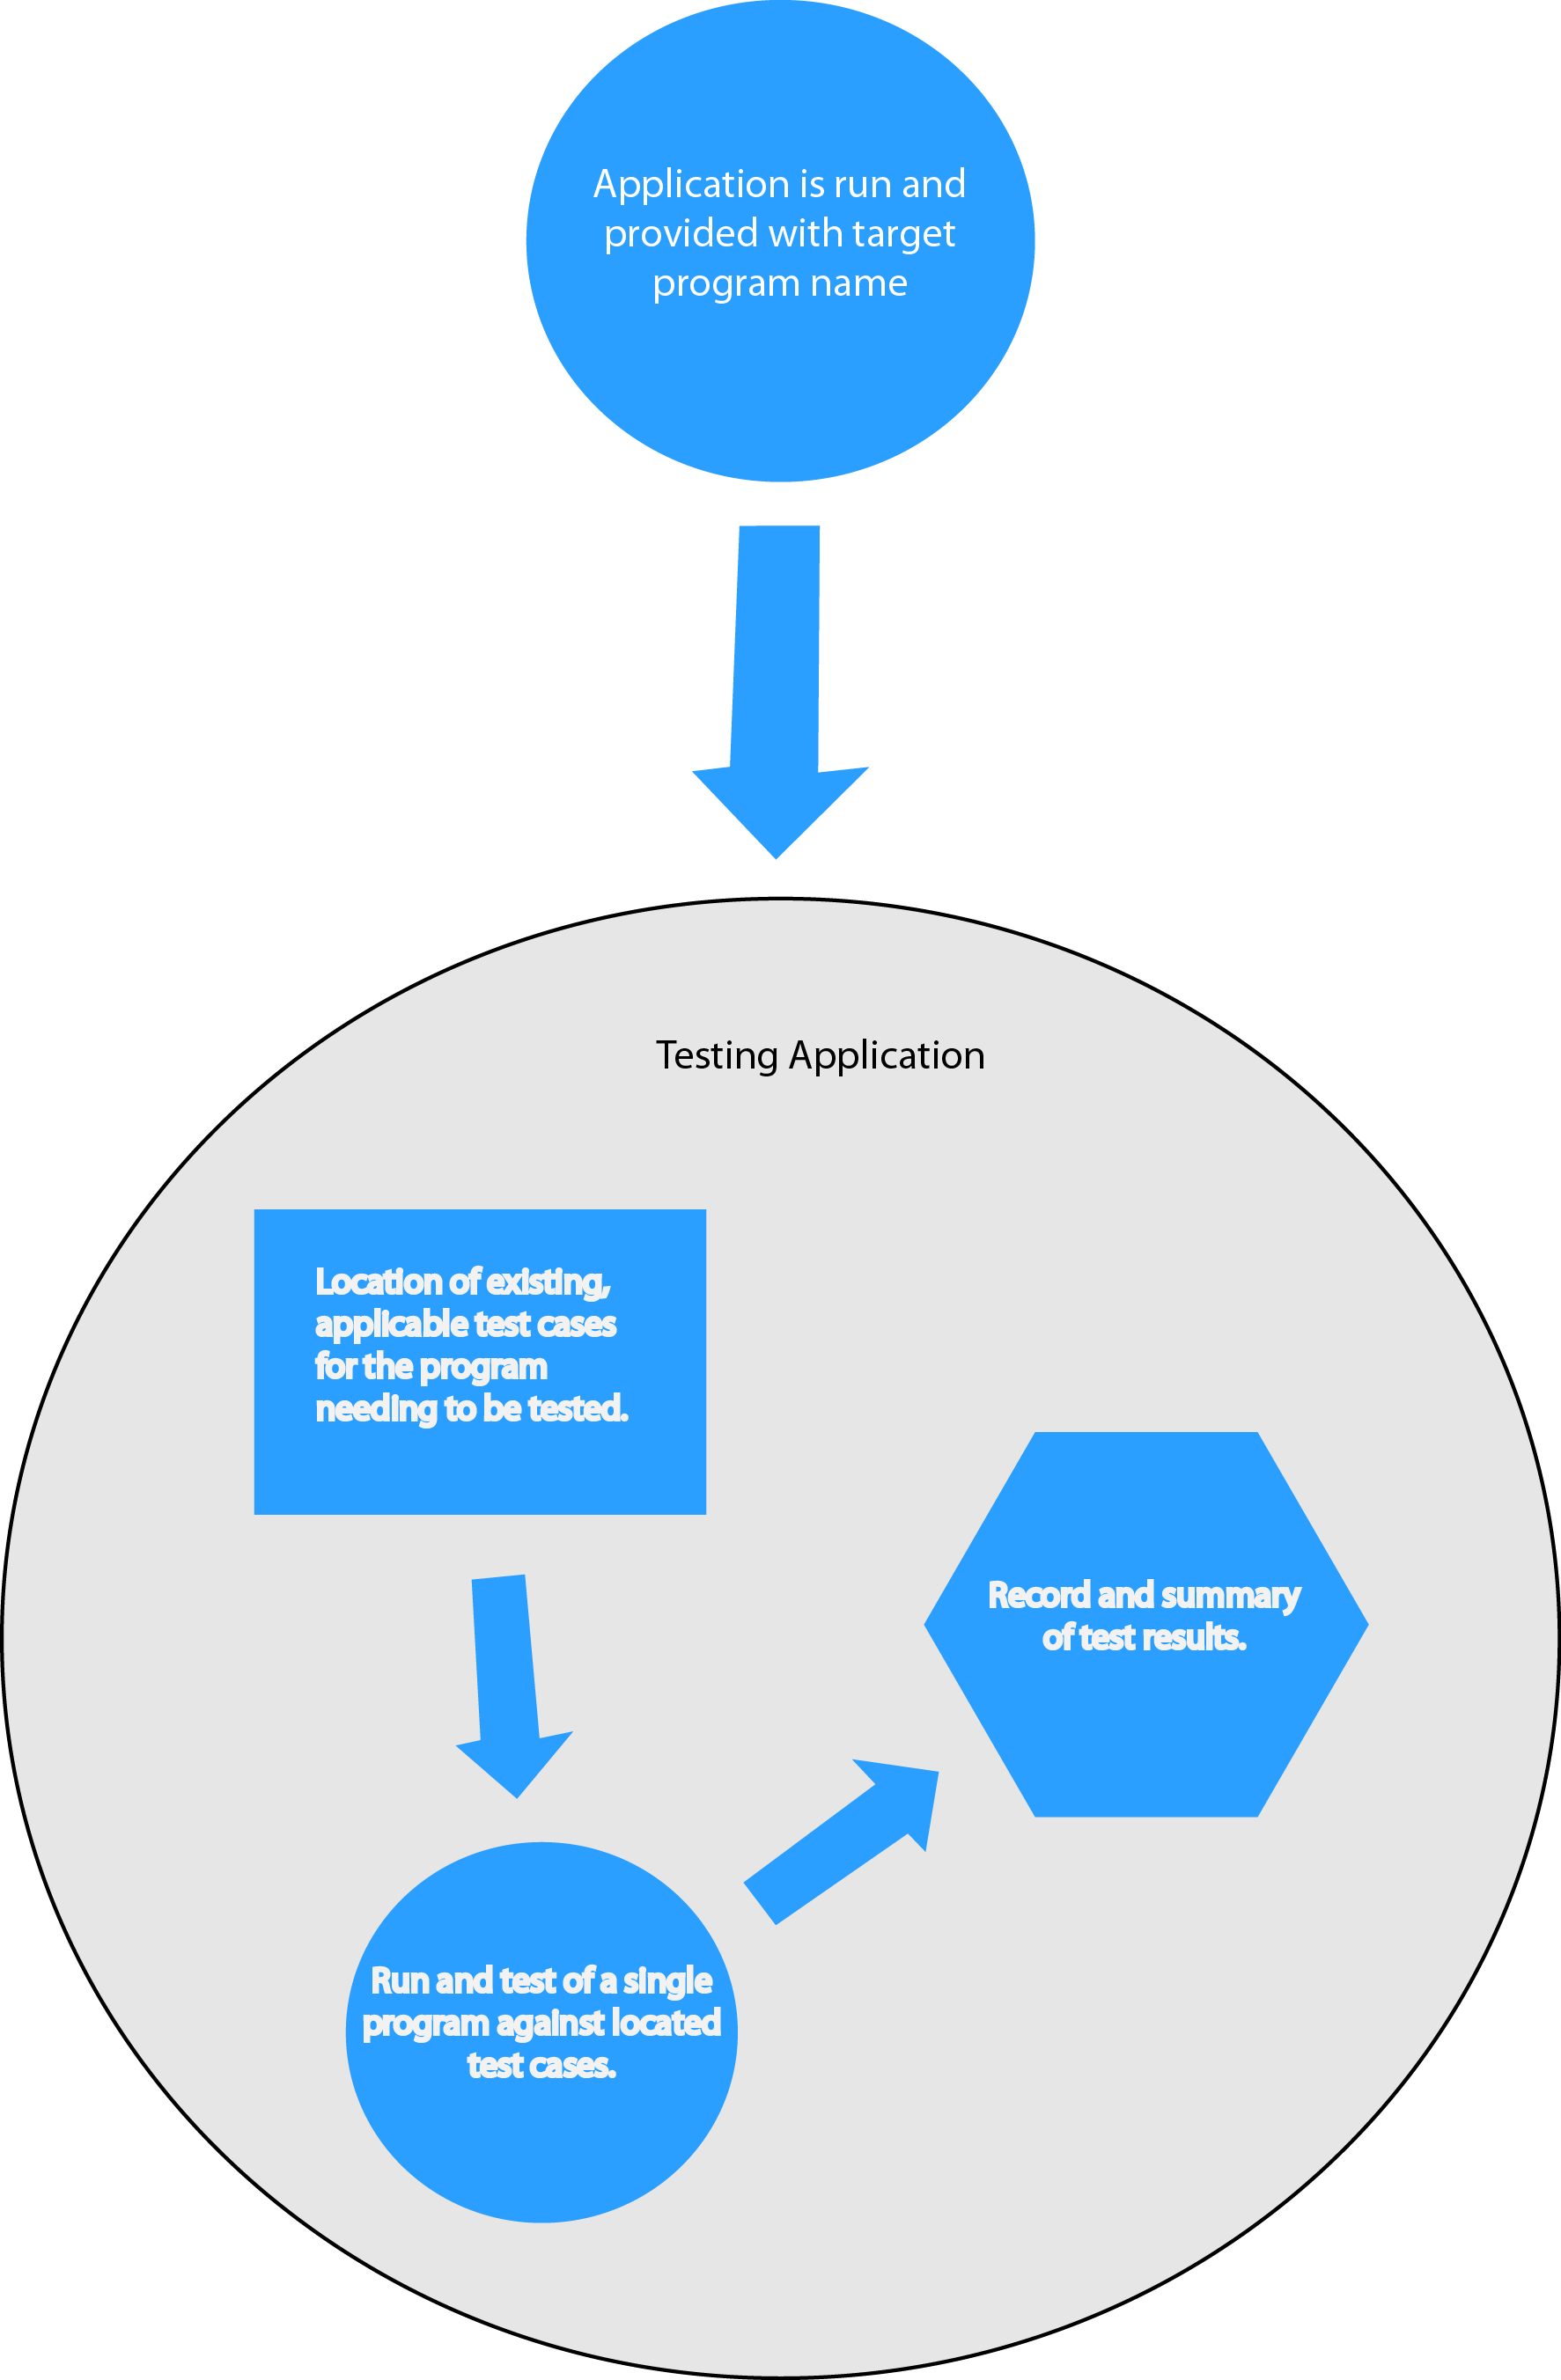
\includegraphics[width=0.9\textwidth]{./diagram}
\end{center}
\caption{The Testing System Diagram \label{systemdiagram}}
\end{figure}



\section{Technologies Overview}
The development team used the Agile Software Development Method, via the Scrum framework, to develop
this system.  This incremental development menthod was the required development method for this project.
Since the system was expected to created for a Linux platform, it was written and tested on a Linux Platform 
using Qt Creator.  The latter was picked as the Integrated Development Environment of the system, based on
the requirement that it be written in the programing language C++.
See Table~\ref{DevelopmentTable}.  
\begin{table}[tbh]
\begin{center}
\begin{tabular}{|r|l|}
  \hline
  Software Development Method & Agile Software Development Method \\
  Planning and Organization & Trello Project Management Application \\
  \hline \hline
  Platform & Linux \\
  Language & C++ \\  
  IDE & Qt Creator \\
  Version Control & Git and Bitbucket
  \\ \cline{2-2}
  
  \hline
\end{tabular}
\caption{The Development Methods and Technologies Table \label{DevelopmentTable}}
\end{center}
\end{table}

